\chapter{Implementation and Validation}

For a detailed description of specific functions etc., see the comments in the actual code. The general idea of the implementation is to use the power of object orientation (for details, see Section~\ref{sec:OO}) to compile the different building blocks of QMC-methods in a natural coherent way. The first step to accomplishing this is to extract the different (more or less) independent parts of the machinery.

\section{Structure and Implementation}
\label{sec:StructureandImplementation}

In QMC, and Quantum Mechanics in general, there are several natural ways of decoupling the code. Gathering data into objects are in some cases done to increase the readability and the overall structure, which dramatically decreases the time it takes to implement or debug new methods. Another reason is to generalize the code for several different cases, without having to rewrite or mess up anything (see the PotionGame example in Section~\ref{sec:PotionGame}).

\subsection{Methods used for Increasing Readability and Overall Structure}

As an example, take a look at the contents of the Walker class in Table ~\ref{tab:walkerClassMembers}. The power of this way of structuring the code, is that whenever we need a new walker in e.g. DMC, all we need to do is to create a new instance of \verb+Walker+. A function which requires access to several elements from Table~\ref{tab:walkerClassMembers} now only requires one argument, namely the walker of interest. Let us look at an example

\begin{table}
\label{tab:walkerClassMembers}
\begin{center}

\caption{Description of the members in an instance of the Walker class. All matrices holds information on all particles.}

 \begin{tabular}{|l| c l|}
 \hline
 \verb+arma::mat r+           &  & The position.\\
 \verb+arma::mat r_rel+       &  & The relative positions.\\
 \verb+arma::rowvec r2+       &  & The squared positions. \\
 \verb+arma::mat qforce+      &  & The quantum force.\\
 \verb+arma::mat spatial_grad+&  & The gradient of the uncorrelated wave function.\\
 \verb+arma::mat jast_grad+   &  & The gradient of the Jastrow factor.\\
 \verb+arma::mat inv+         &  & The inverse of the slater matrix.\\
 \verb+double spatial_ratio+  &  & The current ratio between this walker and another walker.\\
 \verb+double value+          &  & The value of the wave function.\\
 \verb+double lapl_sum+       &  & The full Laplacian of the wave function.\\
 \verb+double E+              &  & The energy of the walker. \\
 \verb+bool is_murdered+      &  & False if active, true if not. \\
 \hline 
 \end{tabular}
 
 
\end{center}
\end{table}


\vspace{0.5 cm}
\begin{lstlisting}
DMC::DMC(...) {

    ...
 
    int max_walkers = K * n_w;
    original_walkers = new Walker*[max_walkers];
    
    ...

}
\end{lstlisting}


\begin{lstlisting}
void DMC::initialize() {

    jastrow->initialize();

    //Initializing active walkers
    for (int k = 0; k < n_w; k++){
        original_walkers[k] = new Walker(n_p, dim);
    }
    
    //Seting trial position of active walkers
    ...

    //Calculating and storing energies of active walkers
    for (int k = 0; k < n_w; k++) {
        calculate_energy_necessities(original_walkers[k]);
        original_walkers[k]->set_E(calculate_local_energy(original_walkers[k]));
    }

    //Creating unactive walker objects (note: 3. arg=false implies dead) 
    for (int k = n_w; k < K * n_w; k++) {
        original_walkers[k] = new Walker(n_p, dim, false);
    }

}
\end{lstlisting}

\begin{lstlisting}
Walker::Walker(int n_p, int dim, bool alive) {
    this->dim = dim;
    this->n_p = n_p;
    this->n2 = n_p / 2;


    if (alive) {
        is_murdered = false;
    } else {
        is_murdered = true;
    }
    
    r = zeros<mat > (n_p, dim);
    r_rel = zeros<mat > (n_p, n_p);
    qforce = zeros<mat > (n_p, dim);
    jast_grad = zeros<mat > (n_p, dim);
    spatial_grad = zeros<mat > (n_p, dim);

    r2 = zeros(1, n_p);

    value = 0;
    lapl_sum = 0;
    spatial_ratio = 0;
    inv = zeros<mat > (n2, n_p);

}
\end{lstlisting}

As we can see from the code above, initializing new walkers is unproblematic. When e.g. looping over walkers in DMC, the amount of juggling is reduced to nothing; all you need to do is to loop over an array of walkers. This walker can then be sent to any function, resulting in code like e.g.

\vspace{0.5cm}
\begin{lstlisting}
double Coulomb::get_pot_E(const Walker* walker) const {
    
    double e_coulomb = 0;

    for (int i = 0; i < n_p - 1; i++) {
        for (int j = i + 1; j < n_p; j++) {
            e_coulomb += 1 / walker->r_rel(i, j);
        }
    }

    return e_coulomb;
}
\end{lstlisting}

The alternative to the code above is to juggle one relative position matrix per walker, ruining both the readability and the overall structure of the code. Another upside to this way of structuring, is that we can tie the source code and the method description closer together. Look at VMC as an example. Stating e.g. that at cycle zero, the original and trial walker should be equal, is now implemented in the following way:

\vspace{0.5cm}
\begin{lstlisting}
void VMC::initialize() {
    
    ...

    sampling->set_trial_pos(original_walker);
    copy_walker(original_walker, trial_walker);
}

\end{lstlisting}

Another example where object orientation dramatically increases the readability of the code is the interplay between the Sampling- and Diffusion-class. From \textbf{REF TO THEORY} we know that if we use importance sampling, the diffusion follows the Fokker-Planck equation (Eq.~\textbf{CITE EQ FOKKERPLANCK}). The implementation is as follows:

\vspace{0.5cm}
\begin{lstlisting}
Importance::Importance(int n_p, int dim, double timestep, long random_seed, double D)
: Sampling(n_p, dim) {
    diffusion = new Fokker_Planck(n_p, dim, timestep, random_seed, D);
}
\end{lstlisting}


\subsection{Methods for Generalizing the Code}

The importance sampling constructor serves as a good example in this case as well. A \verb+Sampling+ object type might be an instance of \verb+Importance+ or \verb+Brute_Force+, however, we do not need to know this in order to diffuse a walker. We do not even need to know whether we are doing VMC or DMC. All we need to know is that the \verb+Diffusion+ object within the sampling will give us the values we need once the correct objects are in place. This is reflected in the following code:

\vspace{0.5cm}
\begin{lstlisting}
void QMC::update_pos(const Walker* walker_pre, Walker* walker_post, int particle) const {

    for (int j = 0; j < dim; j++) {
        walker_post->r(particle, j) = walker_pre->r(particle, j)
                + sampling->get_new_pos(walker_pre, particle, j);
    }
    
    ...
    
}
\end{lstlisting}

\begin{lstlisting}
double Sampling::get_new_pos(const Walker* walker_pre, int particle, int j) const {
    return diffusion->get_new_pos(walker_pre, particle, j);
}
\end{lstlisting}

\begin{lstlisting}
double Diffusion::get_new_pos(const Walker* walker, int i, int j) {
    return gaussian_deviate(&random_seed) * std;
}

...

double Simple::get_new_pos(const Walker* walker, int i, int j) {
    return Diffusion::get_new_pos(walker, i, j);
}

...

double Fokker_Planck::get_new_pos(const Walker* walker, int i, int j) {
    return D * timestep * walker->qforce(i, j) + Diffusion::get_new_pos(walker, i, j);
}
\end{lstlisting}

This use of virtual functions to generalize the code is used throughout the entire code. The goals of this thesis was to produce a code with the following generalizations:

\begin{itemize}
 \item As many as possible functions should be written generally for DMC and VMC (see Section~\textbf{REF} for a complete list of the common parts.)
 \item Objects should not assume the type of any sub-classed object except its own, unless the type is directly implied (importance sampling implies Fokker-Planck diffusion).
\end{itemize}

This puts a series of constraints on the code; it should be general for:

\begin{enumerate}[label=(\roman{*}), ref=(\roman{*})]
\item Importance- and Brute Force-sampling.
\item Numerical or closed form expressions for the kinetic energy and quantum force.
\item Fermions and Bosons.
\item Any choice of single particle basis.
\item Functionality to add any potential.
\end{enumerate}

It is also implemented a general Jastrow factor, a Walker class which is easily extendable, and an output function which performs any form of output (or nothing), without having to flag / comment the code (it works in a similar way to how QMC extracts potential energies, which will be discussed later). 

\subsubsection{Constraints (i) - (iii)}

As discussed in the beginning of this chapter, \verb+QMC+ holds an object of type \verb+Sampling+, which holds all the functions for moving particles, and ensures that the walker has access to the correct necessities prior to e.g. the energy calculations (which again is different for \verb+Numerical+ or \verb+Closed_Form+). Below follows a part of the code illustrating this; the code for copying walkers, calculating energy necessities etc. follows the same idea.

\vspace{0.5cm}
\begin{lstlisting}
void QMC::update_pos(const Walker* walker_pre, Walker* walker_post, int particle) const {

    //position updated
    ...
      
    sampling->update_necessities(walker_pre, walker_post, particle);

}
\end{lstlisting}

\begin{lstlisting}
void Brute_Force::update_necessities(const Walker* walker_pre, Walker* walker_post, int particle) {
    qmc->get_wf_value(walker_post);
}

...

void Importance::update_necessities(const Walker* walker_pre, Walker* walker_post, int particle) {
    qmc->get_kinetics_ptr()->update_necessities_IS(walker_pre, walker_post, particle);
    qmc->get_kinetics_ptr()->get_QF(walker_post);
}
\end{lstlisting}

\begin{lstlisting}
void Numerical::update_necessities_IS(const Walker* walker_pre, Walker* walker_post, int particle) const {
    qmc->get_wf_value(walker_post);
}

...

void Closed_form::update_necessities_IS(const Walker* walker_pre, Walker* walker_post, int particle) const {
    walker_post->spatial_ratio = qmc->get_system_ptr()->get_spatial_ratio(walker_pre, walker_post, particle);
    qmc->get_system_ptr()->calc_for_newpos(walker_pre, walker_post, particle);
    qmc->get_gradients(walker_post, particle);
}
\end{lstlisting}

\begin{lstlisting}
double Fermions::get_spatial_ratio(const Walker* walker_pre, const Walker* walker_post, int particle) const {
    int q_num;
    double s_ratio;

    s_ratio = 0;
    for (q_num = 0; q_num < n2; q_num++) {
        s_ratio += orbital->phi(walker_post, particle, q_num) * walker_pre->inv(q_num, particle);
    }

    return s_ratio;
}

...

void Fermions::calc_for_newpos(const Walker* walker_old, Walker* walker_new, int particle) const {
    update_inverse(walker_old, walker_new, particle);
}



BOSONS NOT IMPLEMENTED
\end{lstlisting}


We can see that the branching goes as follows (corresponding if-test hierarchy pseudo-code):

\begin{lstlisting}[language=Matlab]
if BF:
    Calculate new wavefunction (fermion = slater, boson = bosonic)
else if IS:
    if Numerical Kinetics:
	Calculate new wavefunction
	
    else if Closed Form Kinetics:
	Get new gradients 
	
	if fermions:
	    Calculate slater determinant ratio
	    Update the inverse matrix
	else if bosons:
	    Calculate bosonic wavefunction ratio
	
\end{lstlisting}

Creating this sort of general code without the use of virtual functions is a complete mess of if-tests, whereas object orientation cleans up most of the mess, abstracting the implementation to easily read statements. On top of this, everything itself depends on the choice of single particle basis, which leads us to the next constraint.

\subsubsection{Constraint (iv)}

Not only do we want a given single particle basis, but the constituents of this basis should themselves be allowed to have any form (i.e. be a superposition of another basis). The way this is handled in the code is to have the single particle basis listed as an array or \verb+function+ objects. The purpose of this object is nothing but being initialized and evaluated. An example is the ground state of the harmonic oscillator:

\vspace{0.5cm}
\begin{lstlisting}
Orbitals::Orbitals(int n_p, int dim) {
    this->n_p = n_p;
    this->dim = dim;

    int max_implemented = 15; //for 30 particles
    basis_functions = new function*[max_implemented];
}

...


oscillator_basis::oscillator_basis(int n_p, int dim, double alpha, double w)
: Orbitals(n_p, dim) {

    ...

    basis_functions[0] = new HO_1(this->alpha, w);
    basis_functions[1] = new HO_2(this->alpha, w);
    basis_functions[2] = new HO_3(this->alpha, w);
    ...
}

...

double oscillator_basis::phi(const Walker* walker, int particle, int q_num) const {
    return basis_functions[q_num]->eval(walker, particle);
}
\end{lstlisting}

\begin{lstlisting}
class function {
public:
    function();
    
    virtual double eval(const Walker* walker, int i) const = 0;
};

...

class HO_1 : public function {
protected:
    double* alpha;
    double w;

public:

    HO_1(double* alpha, double w);

    virtual double eval(const Walker* walker, int i) const;
};

...

double HO_1::eval(const Walker* walker, int i) const {
    double r2 = walker->get_r_i2(i);

    double x = walker->r(i, 0);
    double y = walker->r(i, 1);

    double H = 1;
    
    return H * exp(-0.5 * (*alpha) * w * r2);
}
\end{lstlisting}

All orbital files are generated automatically by a Python-script. The reason why, in this case, \verb+alpha+ is a pointer, is so that the value can be changed within orbitals, and then consequently be changed within the function class (a must during minimization). 

However, we can abstract it even more. Implementing a single particle basis expanded in e.g. harmonic oscillator basis functions is more or less trivial in this framework. Following is a pseudo code to illustrate this claim:

\vspace{0.5cm}
\begin{lstlisting}[language=C++]
class Expanded_Functions : public functions{
public:
    Expanded_Functions(int m, file_spesifics);
    virtual double eval(const Walker* walker, int i) const;

protected:
    int m;                     
  
    double* coeffs;            
    function** expanded_basis;
  
};

Expanded_Functions::Expanded_Functions(int m, file_spesifics){
    this->m = m;
    coeffs = new double[m];
    expanded_basis = new function*[m];
  
    expanded_basis[0] = new HO_1(alpha=1, w);
  ...
  
  
    //Load coeffs from file e.g. from Hartree Fock runs
}

double Expanded_Functions::eval(const Walker* walker, int i) const {
    
    double value = 0;
    for (int i = 0; i < m; i++){
	value += coeffs[i]*expanded_basis[i]->eval(walker, i);
    }

    return value;

}
\end{lstlisting}


\subsubsection{Constraint (v)}

When we are loading a set of single particle states, we are loading those who best match the given Hamiltonian of our system. For quantum dots, we load harmonic oscillator states, for atoms we load hydrogen states and so on. Having great flexibility in both the Hamiltonian and the basis functions means the code is easily adaptable to other systems. 

The flexibility in the kinetic term has already been described. The way the code loads potential terms is through a \verb+System+ function 

\vspace{0.5cm}
\begin{lstlisting}
void System::add_potential(Potential* pot) {
    potentials.push_back(pot);
}
\end{lstlisting}

where \verb+potentials+ is a vector of potential pointers. When we extract the potential energy term, we simply iterate over the pointers in the array and call a member function

\vspace{0.5cm}
\begin{lstlisting}
double System::get_potential_energy(const Walker* walker) {
    double potE = 0;

    for (std::vector<Potential*>::iterator pot = potentials.begin(); pot != potentials.end(); ++pot) {
        potE += (*pot)->get_pot_E(walker);
    }

    return potE;
}
\end{lstlisting}

Implementing new potentials is also extremely simple; just have the constructor take reasonable parameters, and implement the expression. All in all the code servers great flexibility on all parts without suffering from if-tests or constituting of several unlinked parts. It takes way longer to develop such a code, but it all pays off when it comes to later implementations or extensions of the library.

\section{Performance Optimizations}

\subsection{RAM use}

VMC uses close to zero memory (RAM); we only have two walkers with each their set of matrices. However, DMC has the potential to use a lot of RAM, as thousands of walkers are allocated. The walkers account for close to all of the RAM used by the methods, as the rest of the framework consist only of a small amount of doubles (8 byte) and integers (4 byte). A short analysis of the RAM spent per \verb+Walker+ object yields

\begin{listliketab}
\storestyleof{itemize}
 \begin{tabular}{l l}
  \textbullet 1 boolean                                        & 1 byte                                \\
  \textbullet 3 integers                                       & 12 bytes                              \\
  \textbullet 3 doubles                                        & 24 bytes                              \\
  \textbullet 4 \verb+n_p+ $\times$ \verb+dim+ matrices        & 32 \verb+n_p+ $\cdot$ \verb+dim+ bytes\\
  \textbullet 1 \verb+n_p+ $\times$ \verb+n_p+ matrices        & 8 \verb+n_p+ $\cdot$ \verb+n_p+ bytes \\
  \textbullet 1 \verb+n_p+ $\times$ \verb+n_p/2+ matrix        & 4 \verb+n_p+ $\cdot$ \verb+n_p+ bytes \\
  \textbullet 1 array of length \verb+n_p+                     & 8 \verb+n_p+ bytes                    \\
  Total:                                                       & 37 + 32 \verb+n_p+ $\cdot$ \verb+dim+ + 12 \verb+n_p+ $\cdot$ \verb+n_p+ + 8 \verb+n_p+ bytes \\
 \end{tabular}
\end{listliketab}

For VMC with 30 particles and quantum dots in 2 dimensions this gives a walker RAM usage of 25 kB, which is practically nothing. For DMC however, we have e.g. 1000 active walkers and 4000 inactive. The inactive ones can be left uninitialized, saving the RAM of all matrix initializations (37 RAM per walker). 

In Figure~\ref{FIG:RAMusageDMC} we see how the RAM usage in a typical DMC calculation scales with the number of particles. For 30 particles, we have approximately 60 MB of RAM spent on walkers. This is still practically nothing compared to the available RAM on modern computers (minimum 2 GB).

\begin{figure}
\label{FIG:RAMusageDMC}
 \begin{center}
  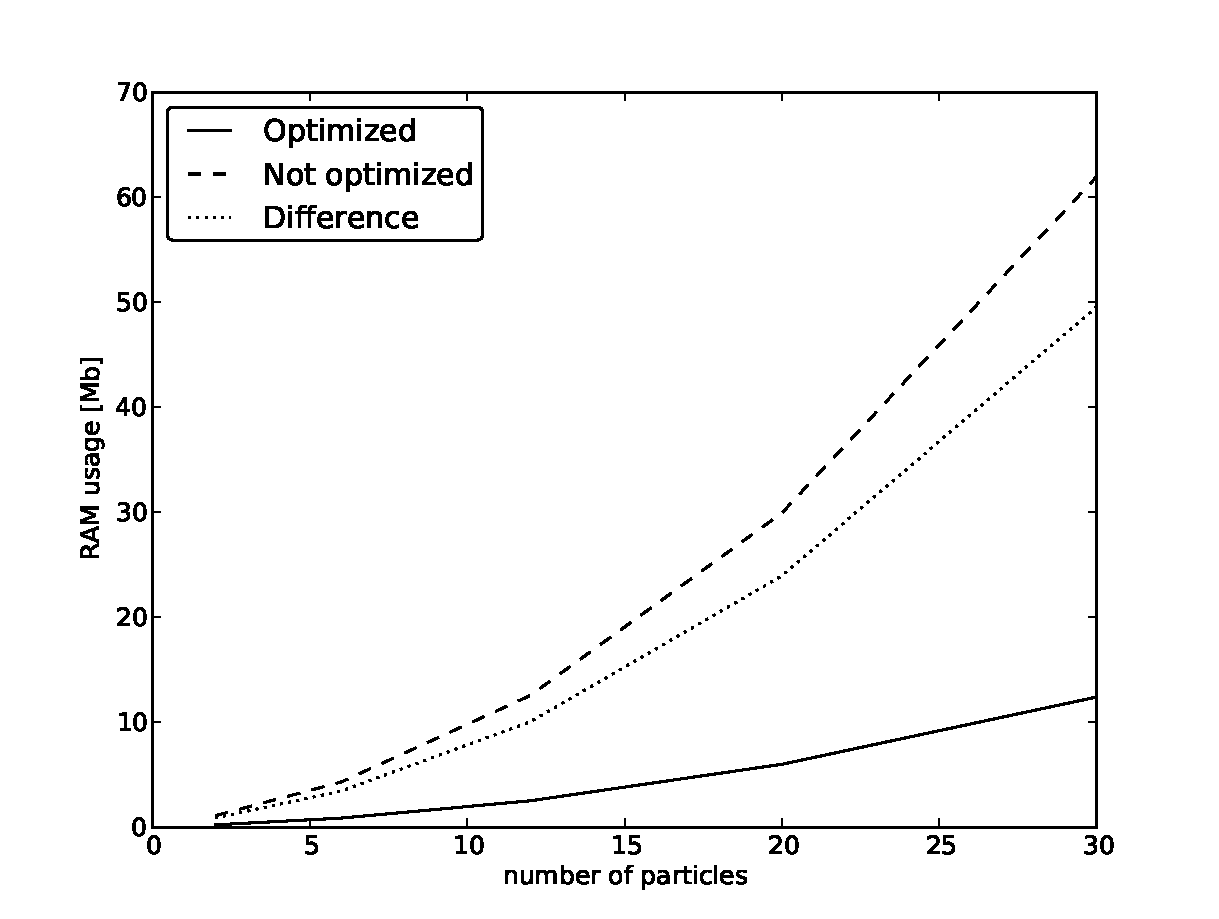
\includegraphics[scale=0.75]{../Graphics/RAMusagePrWalker.pdf}
  \caption{Number of particles vs. the theoretical RAM usage in a typical DMC run for the optimized and unoptimized case. Calculated for two dimensions, 1000 active walkers and 5000 inactive.}
 \end{center}
\end{figure}

The conclusion stands that as long as there are no memory leaks, time spent optimizing the memory use is time wasted. Memory optimizations might damage the readability, so the code was left more or less unoptimized in this part.

\subsection{CPU-time}

During a Quantum Monte Carlo sampling process, certain values, such as the relative distances, are used to calculate quantities such as the energy. The most brute force way of handling situations like this is to calculate everything at the time it is needed. However, once a diffusion step is made,we use the same relative distances both in the Jastrow factor and its gradient. Calculating them twice is a waste of time. We can instead store them in a matrix, and access this matrix in both functions:

\[
r_{rel} = r_{rel}^T = \left( \begin{array}{ccccc}
0 & r_{12} & r_{13} & \cdots & r_{1N} \\
 & 0 & r_{23} & \cdots & r_{2N}  \\
 &  & \ddots & \ddots & \vdots \\
 & \cdots &  & 0 & r_{(N-1)N} \\
 &  &  &  & 0\end{array} \right).
\]

Another upside with this way of storing the relative distances, is that moving particle $i$ in our code, only changes the $i$'th row in the matrix, and therefore we need only to recalculate \textit{N} elements (\textit{N} being the number of particles in our system). For the same reason, storing the gradients, Laplacian sums and the squared radii is matrices also optimize the code. 

Having closed form expressions for the gradients and Laplacians for the different parts of the wave function is another source of dramatic speed-up. The local kinetic energy ($(E_k)_L$) and the Quantum Force ($\mathbf{F}_i$) can be expressed in terms of the separate parts of the wave function:

\begin{eqnarray}
(E_k)_L &=& -\frac{1}{2}\frac{1}{\psi_T}\nabla_i^2 \psi_T \\
&=& -\frac{1}{2}\frac{1}{|S|\psi_C}\nabla_i^2(|S|\psi_C) \nonumber\\
&=& -\frac{1}{2}\frac{1}{|S|\psi_C} \nabla_i \left(\psi_C\nabla_i |S| + |S|\nabla_i \psi_C\right)\nonumber  \\
&=& -\frac{1}{2}\Big[\frac{1}{\psi_C}\nabla_i^2 \psi_C + \frac{2}{|S|\psi_C}\nabla_i|S|\cdot\nabla_i\psi_C \nonumber\\
&& \qquad\qquad\qquad\,\,+\frac{1}{|S|}\nabla_i^2 |S|\Big].\nonumber 
\label{eq:kinetic_analytic}
\end{eqnarray}

\begin{eqnarray}
 \mathbf{F}_i &=& \frac{2}{|S|\psi_C}\nabla_i( |S|\psi_C) \\
&=& 2\left(\frac{1}{\psi_C}\nabla_i \psi_C + \frac{1}{|S|}\nabla_i |S|\right),\nonumber
\label{eq:QF}
\end{eqnarray}
where $i$ denotes particle number, and $|S|$ and $\psi_C$ are respectively the spatial wave function and the Jastrow factor.

For Fermions, it can be shown that we have the following relations for the Slater determinant\cite{larseivind}:

\begin{eqnarray}
 \frac{1}{|S|}\nabla_i |S| &=& \displaystyle\sum_{j=1}^n \nabla_i \phi_j(\vec r_i)S^{-1}_{ji} \\ 
\frac{1}{|S|}\nabla^2_i |S| &=& \displaystyle\sum_{j=1}^n \nabla^2_i \phi_j(\vec r_i)S^{-1}_{ji},\nonumber
\label{eq:grad_lapl_S}
\end{eqnarray}
where $S^{-1}$ is the inverse of the Slater matrix, and $n$ is the dimensionality of the Slater matrix, in our case $n=N/2$, where $N$ is the number of electrons. $\phi_j(\vec r_i)$ are the single-particle basis functions, where $j$ denotes the quantum numbers. For example $j=0$ is the ground state, $j=1$ first excited state and so on. 

These values of the gradient and Laplacian of the single-particle wave functions needs to be tabulated. Most of the single particle bases used are expressed using simple mathematics, such as Hermite polynomials for the case of harmonic oscillator, and the derivatives can therefore be calculated pretty easily. 

Calculating an inverse does not seem to optimize much. However, we can run an updating algorithm for the inverse, which ends up saving a lot of time. The ratio of the spatial determinants can also be expressed using this inverse\cite{larseivind}. This means that no explicit wave function calculation is needed (we can calculate the ratio between two Jastrow factors without problem). The expression for the ratio in terms of the inverse is
\begin{equation}
 R_S = \displaystyle\sum_{j=1}^n \phi_j({\vec r}_{i,\mathrm{new}})S^{-1}_{ji}(\vec r_\mathrm{old}),
\label{eq:Ratio}
\end{equation}
where $i$ is the particle being moved.

In the case of $s=\frac{1}{2}$-Fermions, the code holds two slater determinants (spin up and down); we need two inverse matrices. All if-tests on whether or not to access spin up or down is however avoided by merging the two inverse matrices into one augmented matrix

\[
 S^{-1} = \left[S^{-1}_\uparrow S^{-1}_\downarrow\right].
\]

\noindent
This way of storing the data completely removes the need of if-tests on spin.

Updating the inverse matrix can be done once we got the new position and the ratio

\begin{eqnarray}
 S^{-1}_{kj}(\vec r_\mathrm{new})  = \left\{ 
\begin{array}{l l}
  S^{-1}_{kj}(\vec r_\mathrm{old}) - \frac{1}{R_S}S^{-1}_{ki}(\vec r_\mathrm{old})\displaystyle\sum_{l=1}^{n} \phi_{l}(\vec r_{i,\,\mathrm{new}})  S^{-1}_{lj}(\vec r_\mathrm{old}) &\qquad \mbox{$j \neq i$} \\
 \frac{1}{R_S}S^{-1}_{ki}(\vec r_\mathrm{old})  &\qquad \mbox{$j=i$}
\end{array} \right.
\label{eq:Update_inv}
\end{eqnarray}


Equal expressions like the the ones listed in Eq.~(\ref{eq:grad_lapl_S}) can be found for the case of the Pade-Jastrow factor as well:

\begin{eqnarray}
 \frac{1}{\psi_C^{PJ}}\nabla_i \psi_C^{PJ} &=& \displaystyle\sum_{j\ne i} \frac{\vec r_{ij}}{r_{ij}}\frac{a_{ij}}{(1+\beta r_{ij})^2} \\
\label{eq:grad_jast}
 \frac{1}{\psi_C^{PJ}}\nabla_i^2 \psi_C^{PJ} &=& \left|\frac{1}{\psi_C^{PJ}}\nabla_i \psi_C^{PJ}\right|^2 + 2\displaystyle\sum_{i < j} \frac{a_{ij}(1 - \beta r_{ij})}{r_{ij}(1 + \beta r_{ij})^3}. \nonumber
\label{eq:lapl_jastrow}
\end{eqnarray}

Notice that $a_{ij}$ is written as a matrix element. If we were to calculate $a$ for every single run in the loop, the double if-tests would drain a lot of CPU time. Prior to the sampling, in the \verb+Jastrow::initialize+ function, the values of $a$ are generated once and for all and stored in a matrix. This matrix remains unchanged throughout the entire sampling, and no if-tests are necessary.

For the simplest case of single particle harmonic oscillator basis functions (Eq.~(\textbf{REF OSC BASIS}), the expressions for the derivatives of the wave function with respect to the variational parameters is
\begin{eqnarray}
\frac{1}{\psi_T}\frac{\partial\psi_T}{\partial\alpha} &=& -\frac{1}{2}\omega\displaystyle\sum_{i=1}^N r_i^2, \\
\frac{1}{\psi_T}\frac{\partial\psi_T}{\partial\beta} &=& -\displaystyle\sum_{i<j}\frac{a_{ij}r_{ij}^2}{(1+\beta r_{ij})^2}.
\label{eq:CGM_derivatives}
\end{eqnarray}

which can be used to speed up the process of minimizing.


Optimization (without approximations) is all about not calculating more than you have to. Calculating gradients is the part of the code which require the most CPU time. The most time consuming functions is the gradients. Looking at Eq.~(\ref{eq:grad_lapl_S}) this comes as no surprise; the single particle wave functions contain a call to the exponential function, which is terribly slow and needs to be deadly accurate. The time consumption in the Jastrow gradient arise from the fact that once a particle is moved, the entire gradient changes. 

\section{Validation}

things should not be wrong. It is bad.


test:
\newpage
\begin{table}
\begin{center}
\label{tab:DMCRes}
\begin{tabular}{cc|cccc}
    N     & $\omega$ & $\mathrm{E_{VMC}}$ & $\mathrm{E_{DMC}}$ & $\alpha$ & $\beta$  \\
\hline
    2     &   0.28   & 1.02197  &  1.0216  & 0.970202 & 0.254158 \\
          &   0.5    & 1.66023  & 1.65994  & 0.981901 & 0.312174 \\
          &   1.0    & 3.00054  & 3.00002  & 0.988761 & 0.398956 \\
    6     &   0.28   & 7.62259  & 7.59967  & 0.87322  & 0.322838 \\
          &   0.5    & 11.8092  & 11.7845  & 0.896501 & 0.411444 \\
          &   1.0    & 20.1896  & 20.1606  & 0.920368 & 0.55734  \\
    12    &   0.28   & 25.7088  & 25.63814 & 0.797355 & 0.365122 \\
          &   0.5    & 39.2395  & 39.15974 & 0.859145 & 0.481956 \\
          &   1.0    & 65.7958  & 65.70032 & 0.873605 & 0.656703 \\
\end{tabular}
\caption{J. Hogberget}
\end{center}
\end{table}

\begin{table}
\begin{center}
\label{tab:LohneRes}
\begin{tabular}{cc|cccc}
    N     & $\omega$ & $\mathrm{E_{DMC}}$  \\
\hline
    2     &   0.28   &  N/A     \\
          &   0.5    & 1.65975(2)  \\
          &   1.0    &  3.00000(3) \\
    6     &   0.28   &   7.6001(1) \\
          &   0.5    &  11.7888(2) \\
          &   1.0    &  20.1597(2) \\
    12    &   0.28   &  25.6356(1) \\
          &   0.5    &  39.159(1)  \\
          &   1.0    &  65.700(1)  \\
\end{tabular}
\caption{M. Pedersen Lohne et al.}
\end{center}
\end{table}

\begin{table}
\begin{center}
\label{tab:noColValid}
\begin{tabular}{cc|ccc}
    N     & $\omega$ & $\mathrm{E_{VMC}}$ & $\mathrm{E_{DMC}}$ & $\alpha$ \\
\hline
    2     &   0.5    &   1.0    &   1.0    &   1.0    \\
          &   1.0    &   2.0    &   2.0    &   1.0    \\
    6     &   0.5    &   5.0    &   5.0    &   1.0    \\
          &   1.0    &   10.0   &   10.0   &   1.0    \\
    12    &   0.5    &   14.0   &   14.0   &   1.0    \\
          &   1.0    &   28.0   &   28.0   &   1.0    \\
    20    &   0.5    &   30.0   &   30.0   &   1.0    \\
          &   1.0    &   60.0   &   60.0   &   1.0    \\
    30    &   0.5    &   55.0   &   55.0   &   1.0    \\
          &   1.0    &  110.0   &  110.0   &   1.0    \\
\end{tabular}
\caption{}
\end{center}
\end{table}

